\begin{document}
\begin{appendices}
\setcounter{table}{1}
\setcounter{figure}{0}

\begin{figure}[h]
  \textbf{Conspiracy recommendation networks}\par\medskip
  \centering
  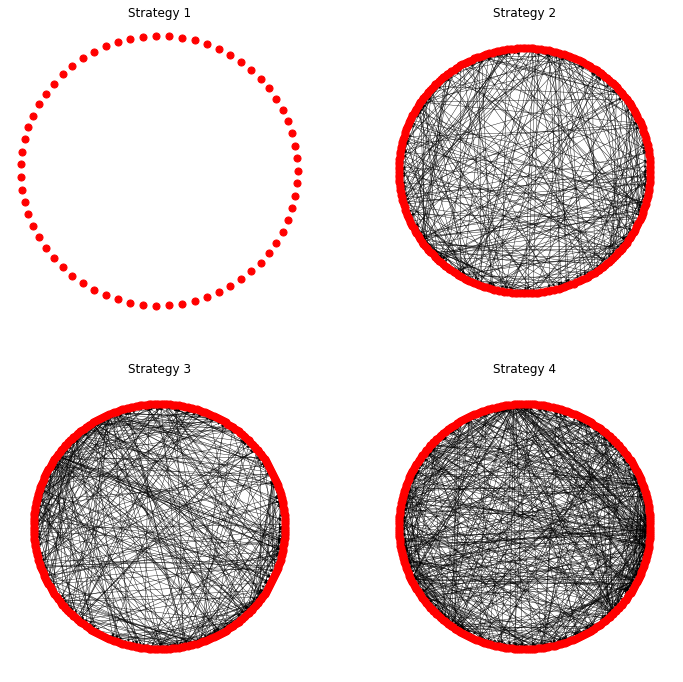
\includegraphics[keepaspectratio, width=\textwidth]{images/conspiracy networks.png}
  \caption{The recommendation networks of each strategy if only conspiracy videos are kept.}
  \label{appendix:networks}
\end{figure}

\begin{figure}
\centering
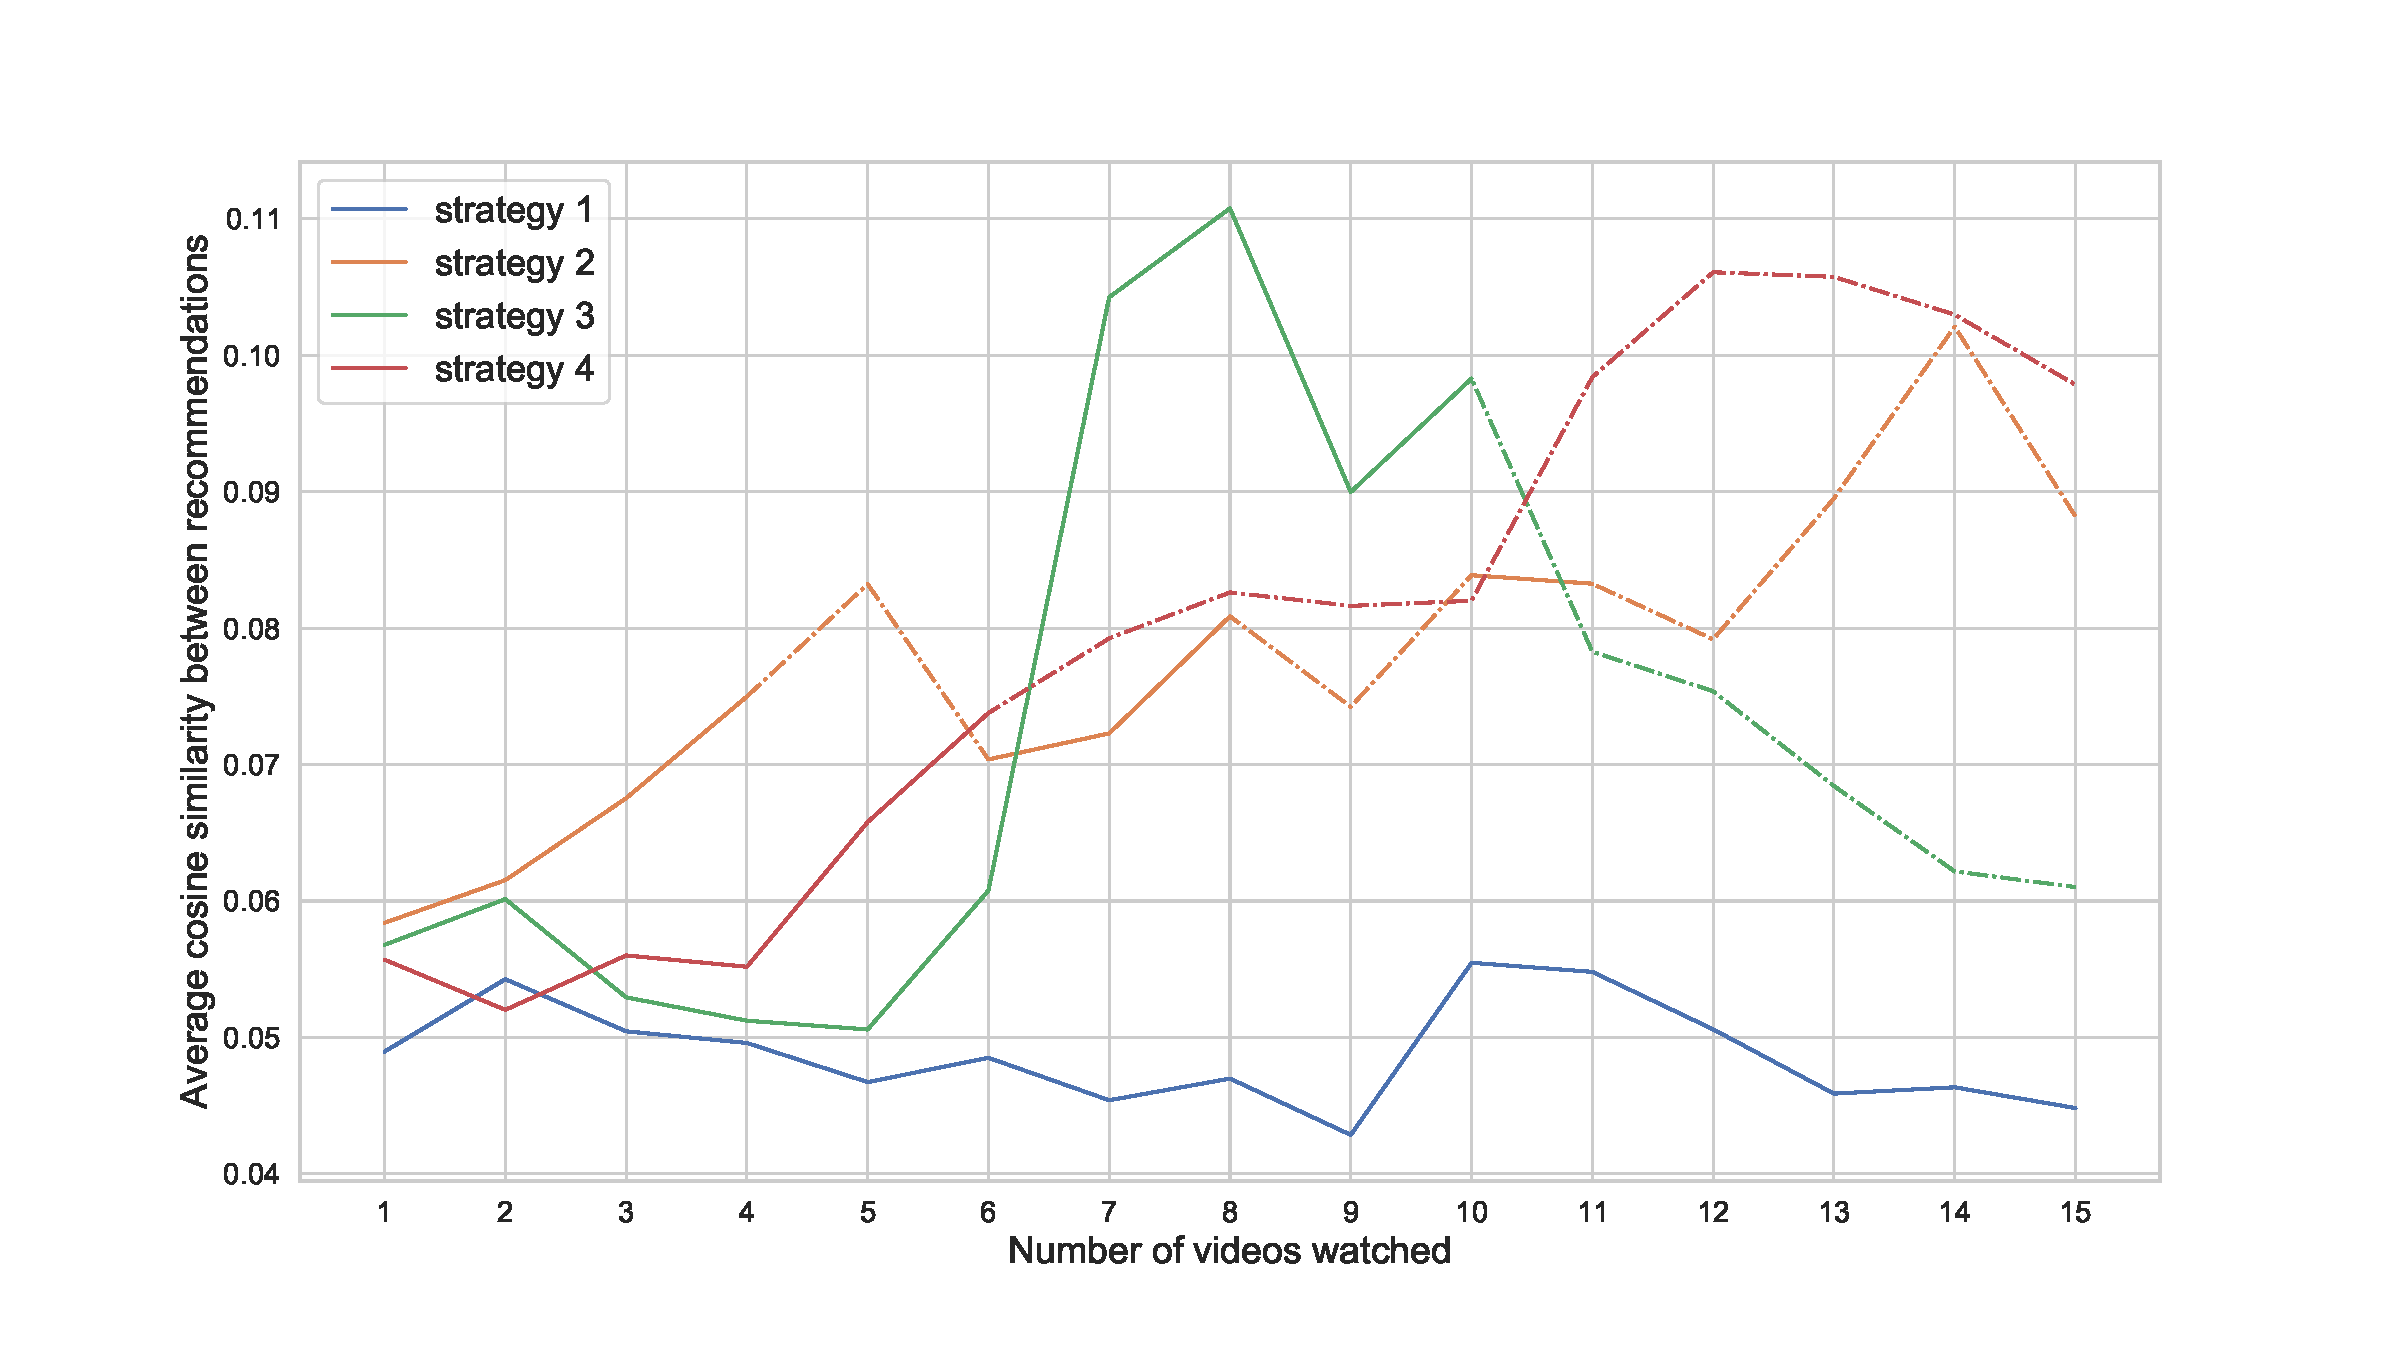
\includegraphics[width=\textwidth]{images/All sim.pdf}
\caption{Cosine similarity of all videos}
\label{appendix:all_sim}
\end{figure}


\begin{figure}
\centering
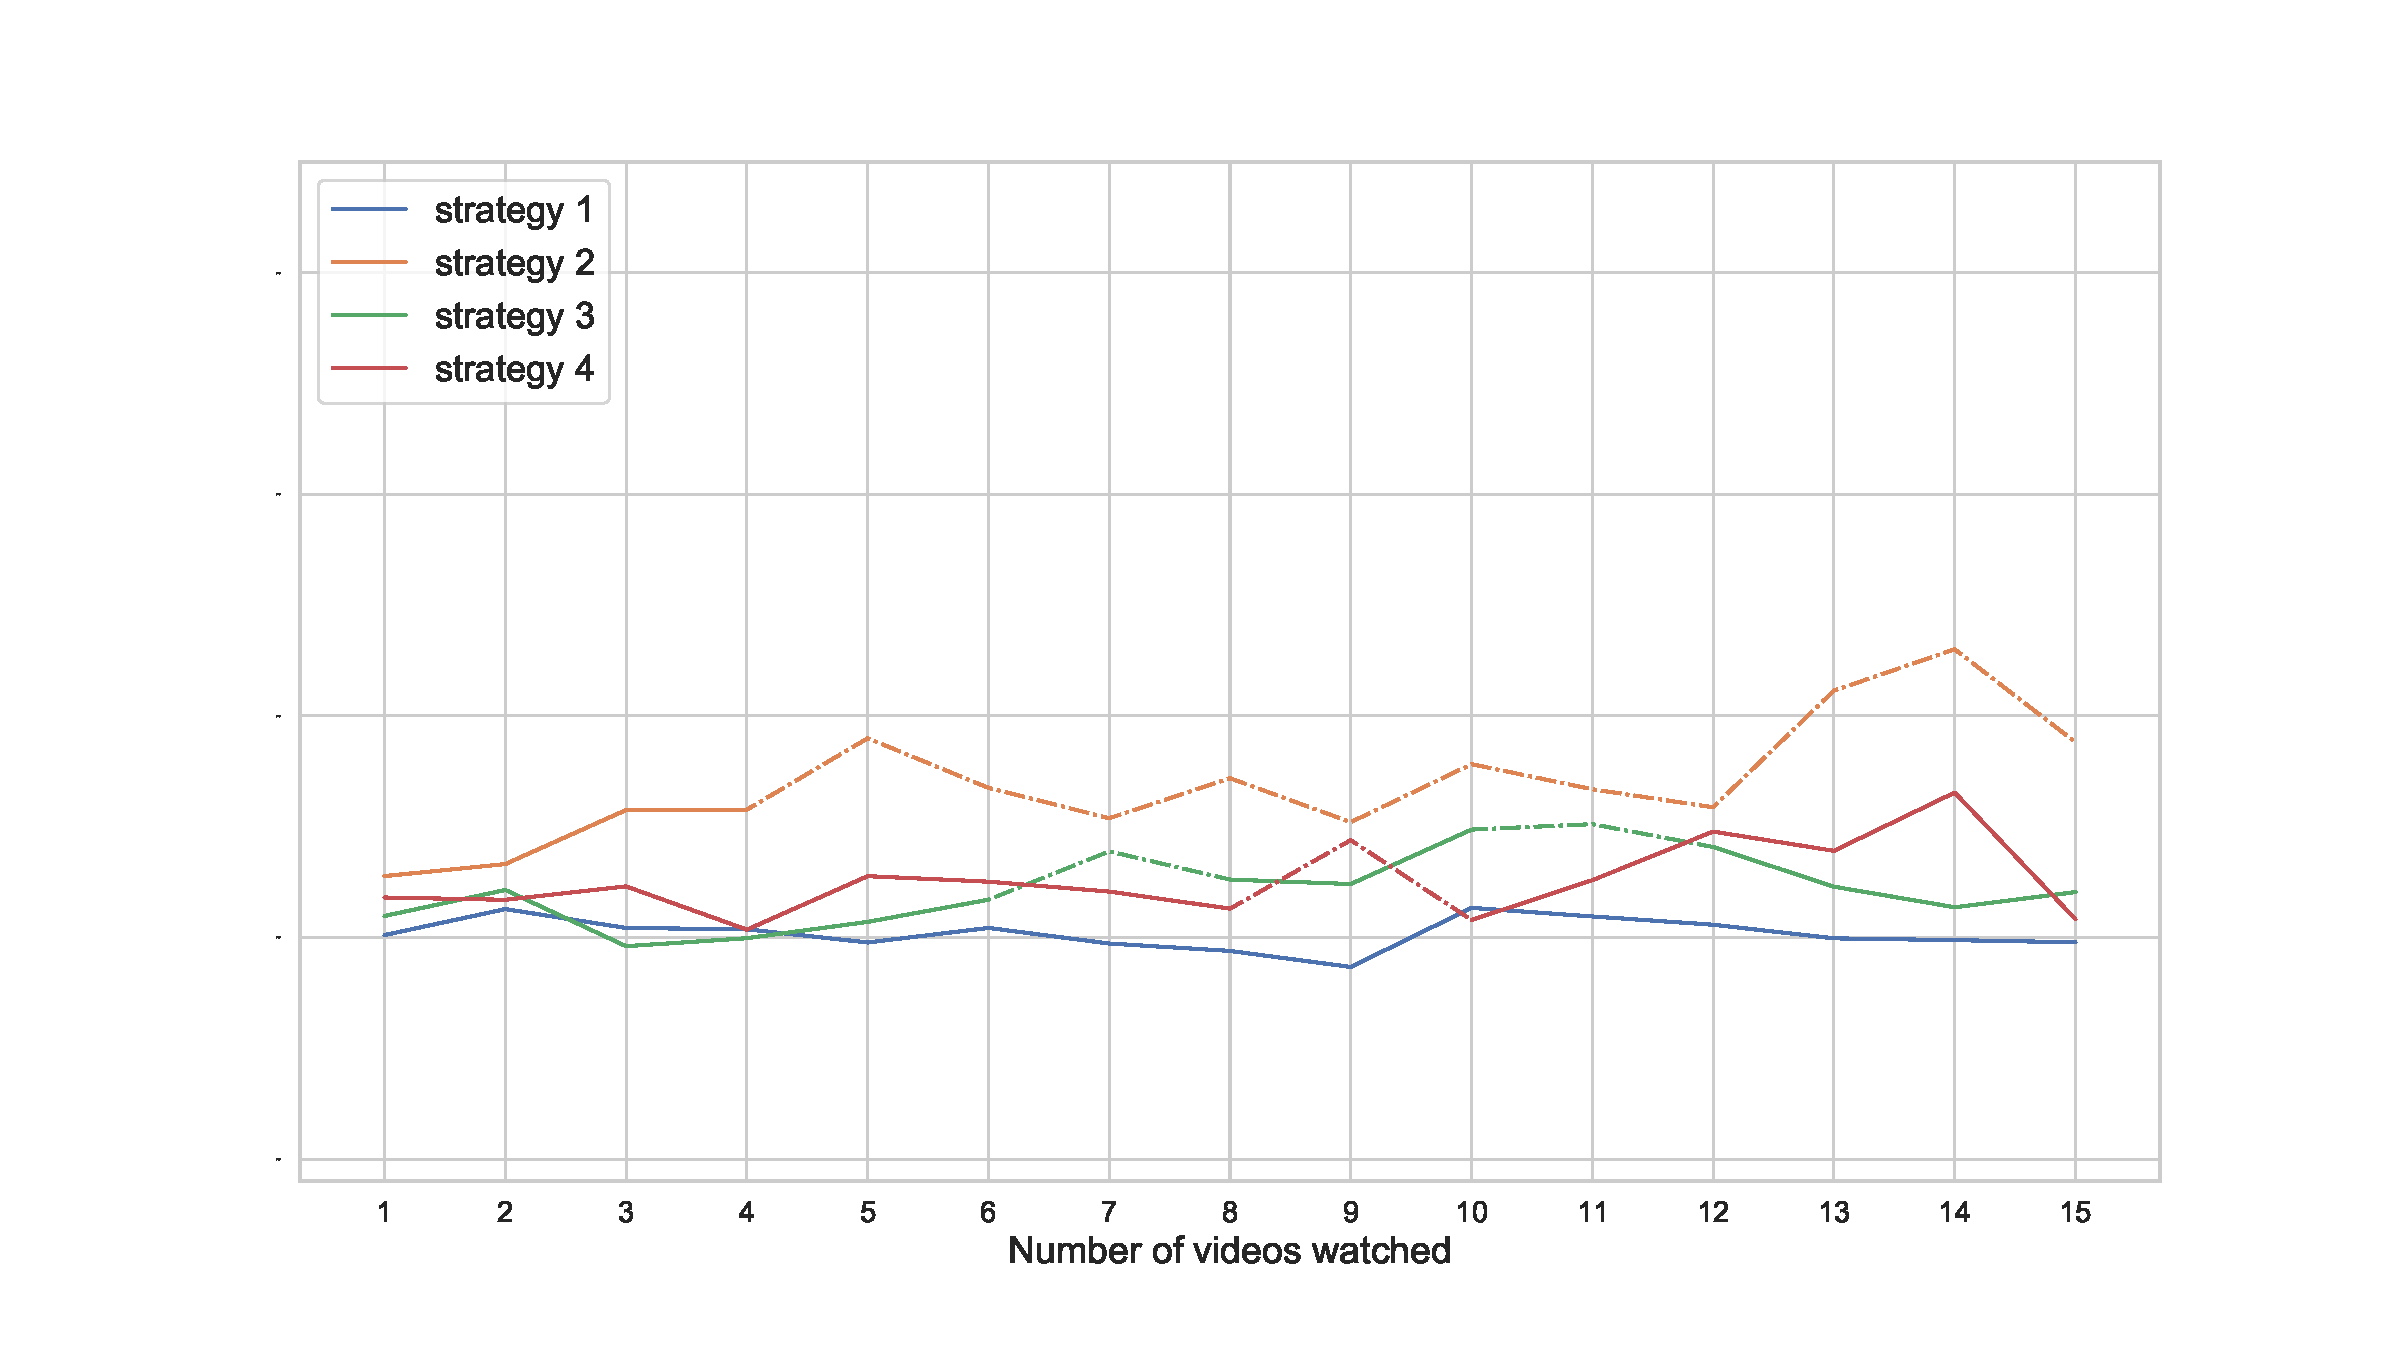
\includegraphics[width=\textwidth]{images/Reg sim.pdf}
\caption{Cosine similarity of regular videos}
\label{appendix:reg_sim}
\end{figure}

\begin{figure}
  \textbf{Average view counts}\par\medskip
  \centering
  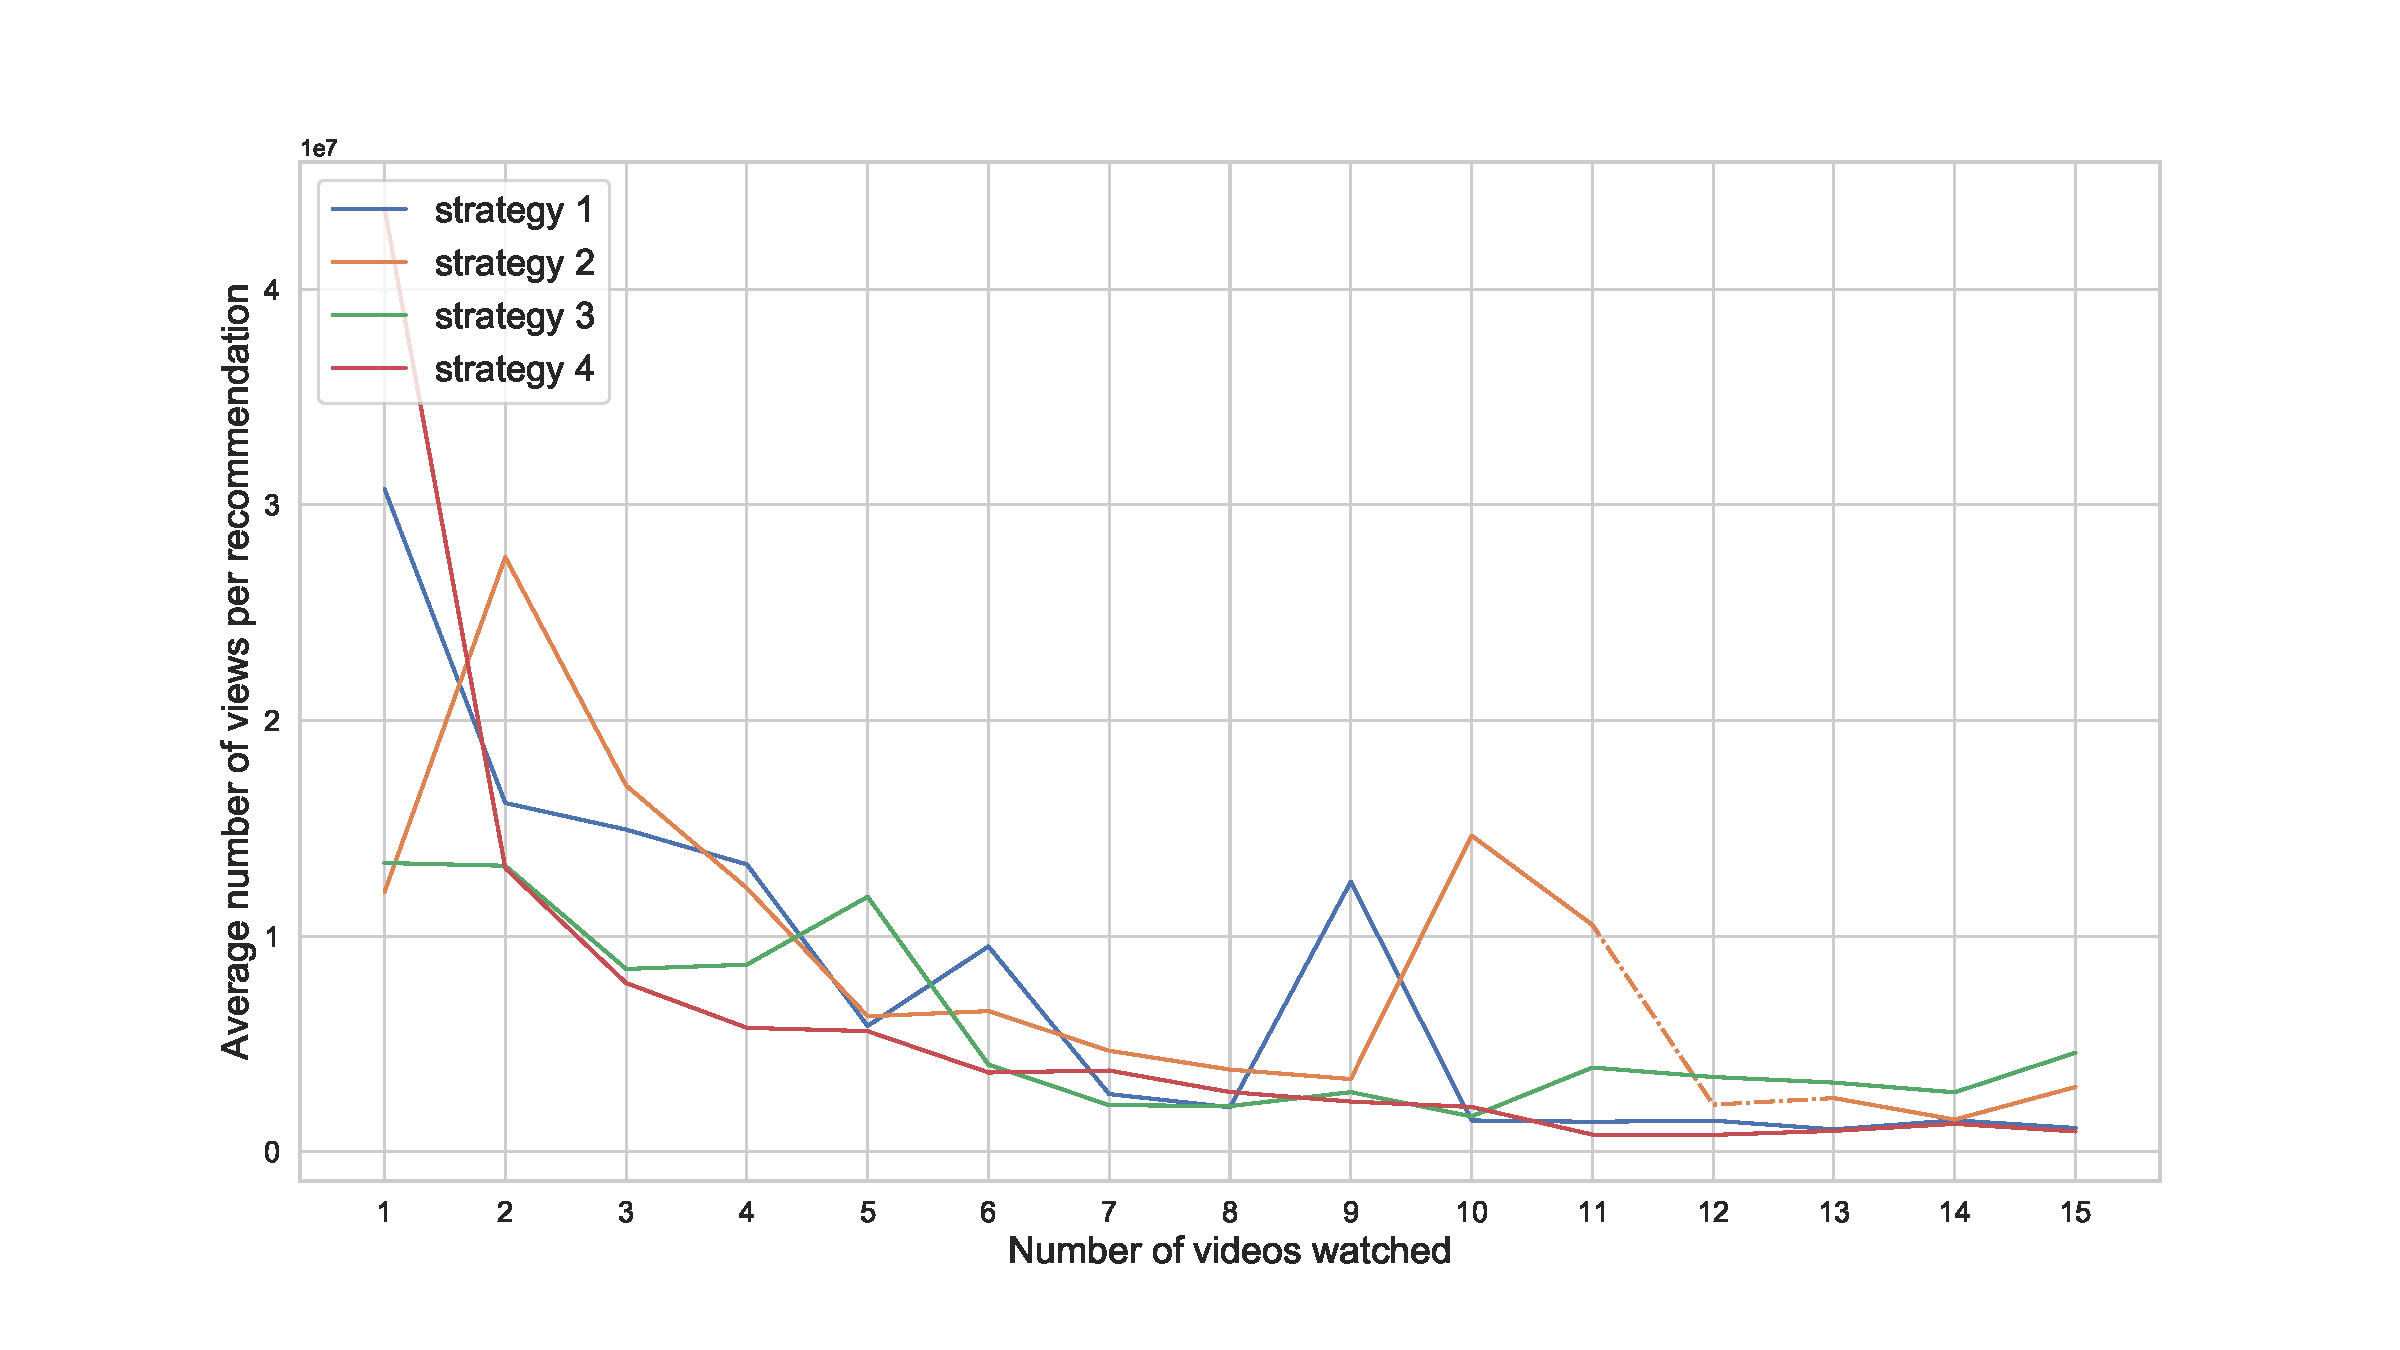
\includegraphics[keepaspectratio, width=\textwidth]{images/views.pdf}
  \caption{The average number of views per recommendation of each watch strategy. Each measure consists of the first twenty recommendations of the five users for each strategy. A dashed line indicates a significant difference compared to the baseline (strategy 1) at $\alpha = 0.05$.}
  \label{appendix:views}
\end{figure}


\begin{figure}
  \textbf{Average video lengths}\par\medskip
  \centering
  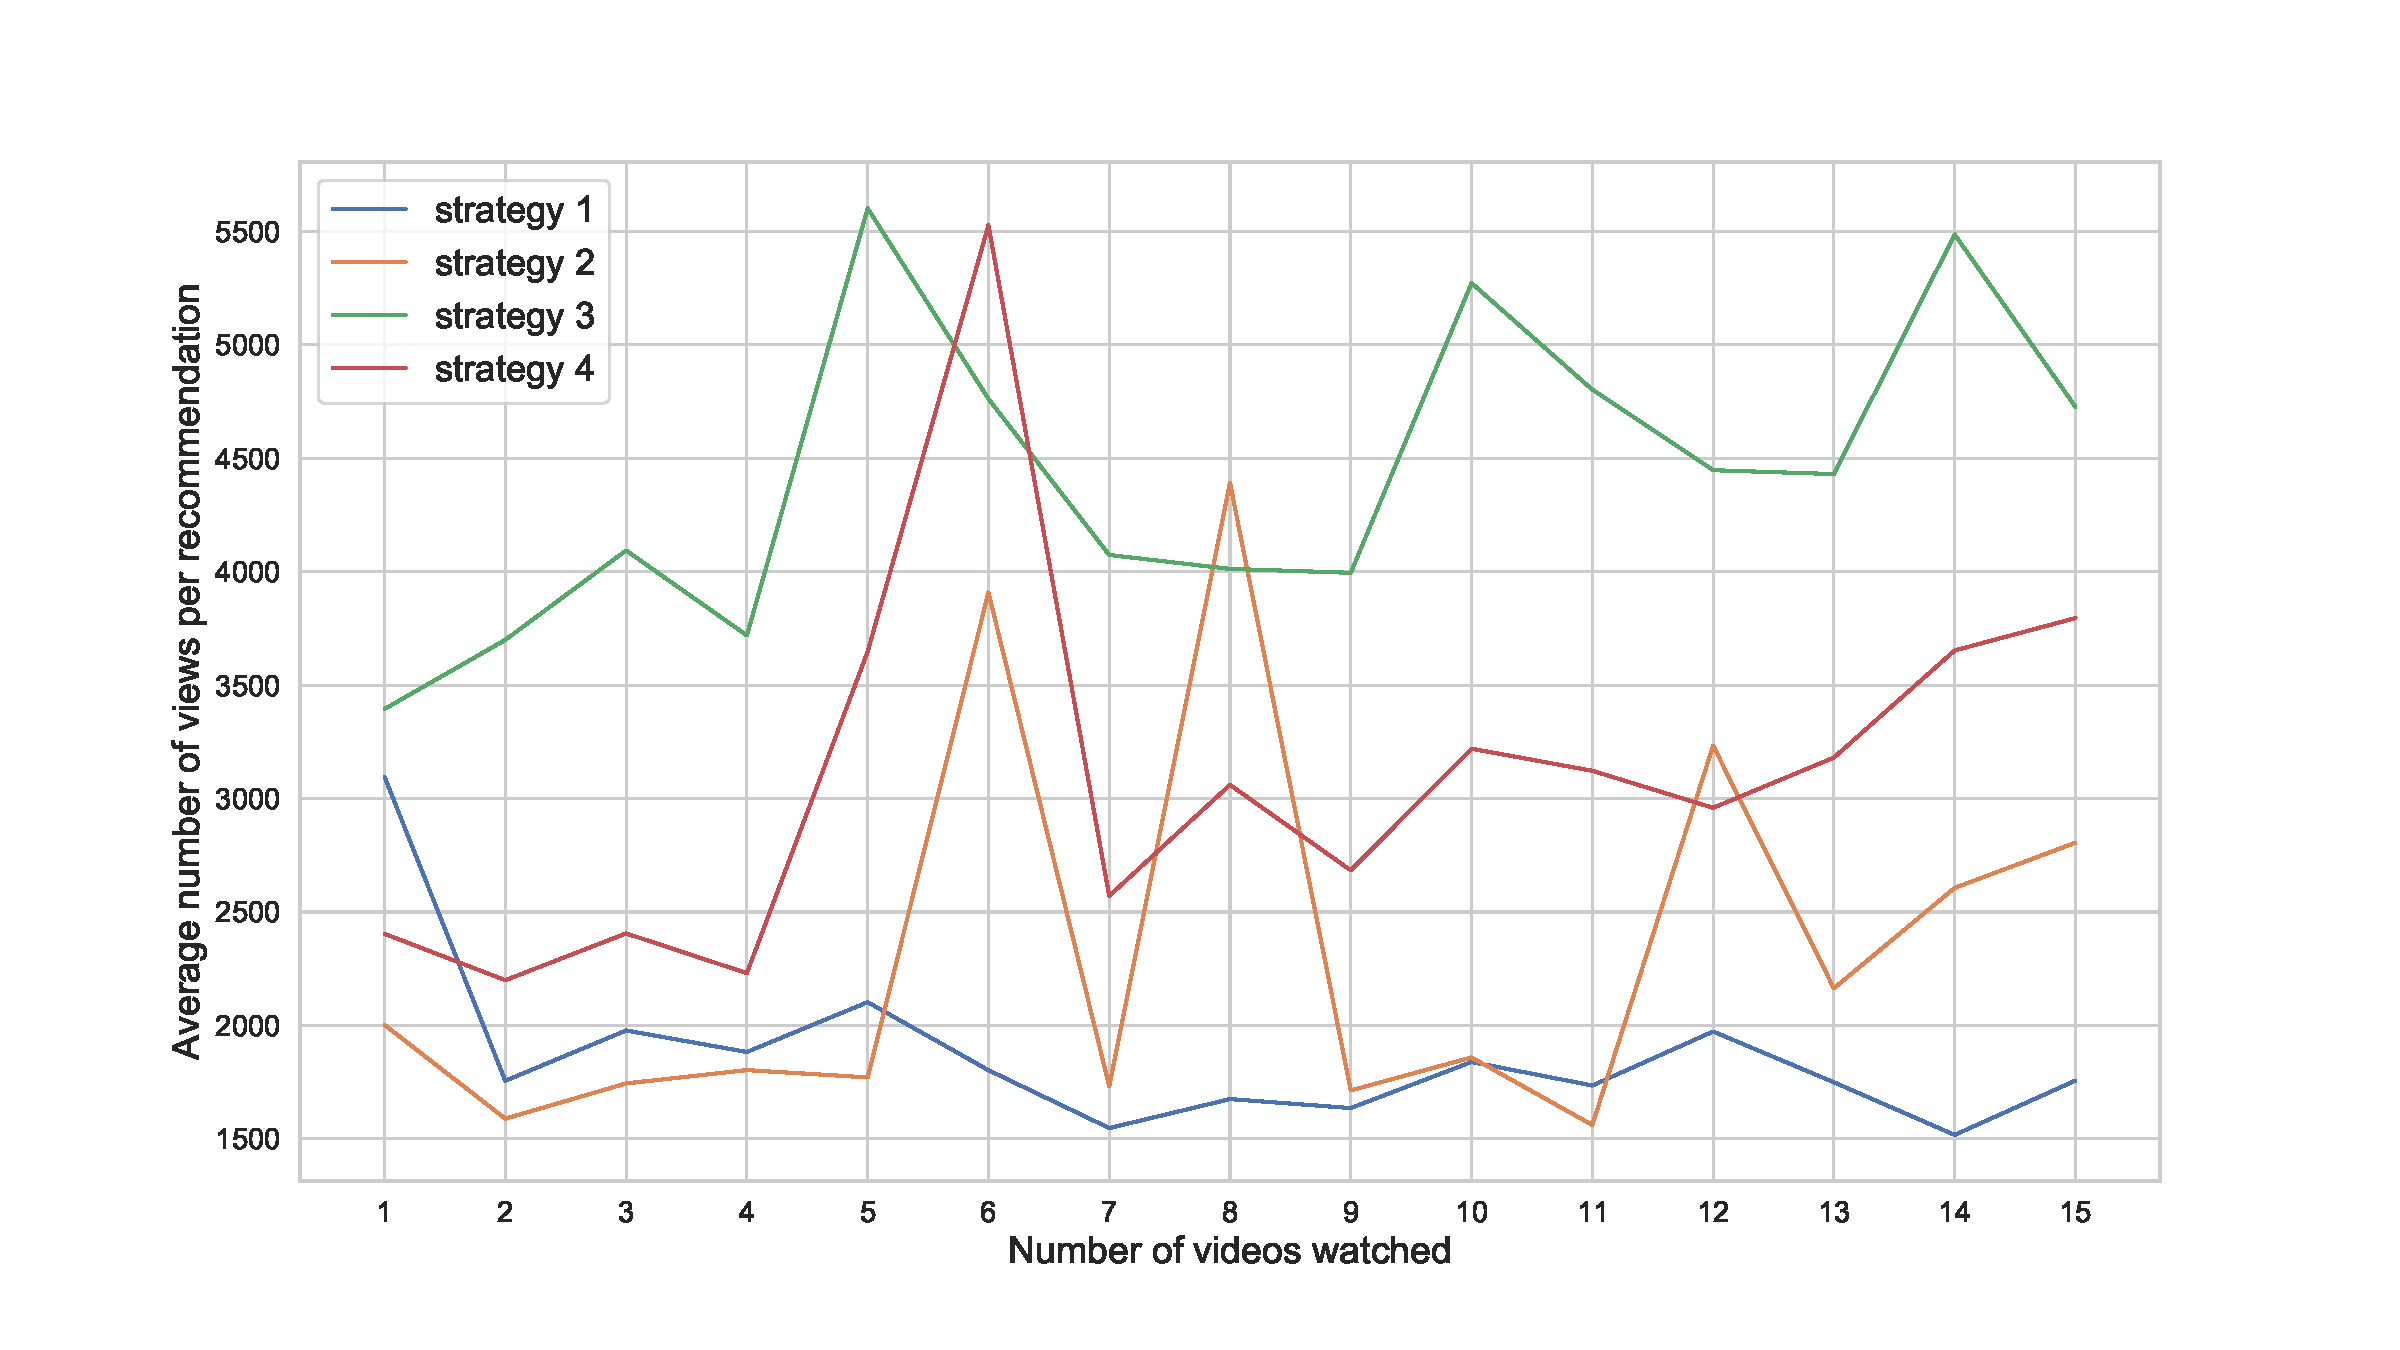
\includegraphics[keepaspectratio, width=\textwidth]{images/durations.pdf}
  \caption{The average duration of the recommendations of each watch strategy in seconds. Each measure consists of the first twenty recommendations of the five users for each strategy. A dashed line indicates a significant difference compared to the baseline (strategy 1) at $\alpha = 0.05$.}
  \label{appendix:durations}
\end{figure}

%%%%%%%%%%%%%%%%%%%%%%%%%%%%%%%%%%%%%%%%%%%%%%%%%%%%%%%%%%%%%%%%%%%%%%%%%%%%%%%%%%%%%%%%%%%%%%%%%%%%%%%

\begin{table}[ht]
\begin{subtable}{\textwidth}
\begin{adjustbox}{minipage=18cm, center}
\sisetup{table-format=-1.5}   
\centering
\begin{tabular*}{\textwidth}{c @{\extracolsep{\fill}} cccccccc}

\toprule
Ensemble     & Activation & Layers        &  Neurons &  Accuracy &  Precision &    Recall &  F1 \\
\midrule
svm, nn, knn &   logistic & 1             &       20 &  \textbf{0.939318} &   \textbf{0.948923} &  \textbf{0.931204} &  \textbf{0.93998} \\
svm, nn, knn &       relu & 1             &       20 &  0.939318 &   0.948923 &  0.931204 &  0.93998 \\
svm, nn, knn &   identity & 1             &        1 &  0.939318 &   0.948923 &  0.931204 &  0.93998 \\
svm, nn, knn &   identity & 10            &        1 &  0.939318 &   0.948923 &  0.931204 &  0.93998 \\
svm, nn, knn &   logistic & 1             &       10 &  0.939318 &   0.948923 &  0.931204 &  0.93998 \\
ridge, svm, nn, knn & tanh & 10           &        1 &  0.939318 &   0.948923 &  0.931204 &  0.93998 \\
svm, nn, knn &       tanh & 1             &       10 &  0.939318 &   0.948923 &  0.931204 &  0.93998 \\
svm, nn, knn &       tanh & 1             &       20 &  0.939318 &   0.948923 &  0.931204 &  0.93998 \\
svm, nn, logr, knn & identity & 1         &        1 &  0.939318 &   0.948923 &  0.931204 &  0.93998 \\
svm, nn, logr, knn & identity & 1         &       10 &  0.939318 &   0.948923 &  0.931204 &  0.93998 \\
\bottomrule

\end{tabular*}
\caption{\label{tab:Ensemble}Ensemble.}
\end{adjustbox}
\end{subtable}

%%%%%%%%%%%%%%%%%%%%%%%%%%%%%%%%%%%%%%%%%%%%%%%%%%%%%%%%%%%%%%%%%%%%%%%%%%%%%%%%%%%%%%%%%%%%%%%%%%%%%%%

\bigskip
\begin{subtable}{\textwidth}
\begin{adjustbox}{minipage=18cm, center}
\sisetup{table-format=-2}   
\centering
\begin{tabular*}{\textwidth}{c @{\extracolsep{\fill}} ccccc}
\toprule
 Kernel &      C &  Accuracy &  Precision &    Recall &        F1 \\
\midrule
    rbf &   10.0 & \textbf{0.936309} &   0.945473 &  0.928747 &  \textbf{0.937035} \\
    rbf &  100.0 &  0.935557 &   0.942289 &  \textbf{0.930713} &  0.936465 \\
    rbf &    1.0 &  0.925276 &   0.930163 &  0.922850 &  0.926492 \\
   poly &   10.0 &  0.916499 &   \textbf{0.946017} &  0.886978 &  0.915547 \\
   poly &  100.0 &  0.915246 &   0.944940 &  0.885504 &  0.914257 \\
 linear &    1.0 &  0.913741 &   0.917944 &  0.912531 &  0.915229 \\
   poly &    1.0 &  0.909729 &   0.935065 &  0.884521 &  0.909091 \\
 linear &   10.0 &  0.904965 &   0.907882 &  0.905651 &  0.906765 \\
 linear &  100.0 &  0.898195 &   0.905830 &  0.893366 &  0.899555 \\
    rbf &    0.1 &  0.878887 &   0.878906 &  0.884521 &  0.881705 \\
\bottomrule
\end{tabular*}
\caption{\label{tab:Support-vector machine}Support-vector machine.}
\end{adjustbox}
\end{subtable}

%%%%%%%%%%%%%%%%%%%%%%%%%%%%%%%%%%%%%%%%%%%%%%%%%%%%%%%%%%%%%%%%%%%%%%%%%%%%%%%%%%%%%%%%%%%%%%%%%%%%%%%

\bigskip
\begin{subtable}{\textwidth}
\begin{adjustbox}{minipage=18cm, center}
\sisetup{table-format=-1.2}   
\centering
\begin{tabular*}{\textwidth }{c @{\extracolsep{\fill}} cccccc}
\toprule
Activation & Layers & Neurons &  Accuracy &  Precision &    Recall &        F1 \\
\midrule
identity   & 10     &      10 &  \textbf{0.923019} &   \textbf{0.935484} &  0.912039 &  \textbf{0.923613} \\
identity   & 25     &      10 &  0.921013 &   0.933031 &  0.910565 &  0.921661 \\
relu       & 10     &      10 &  0.919007 &   0.917561 &  0.924324 &  0.920930 \\
identity   & 10     &      20 &  0.916750 &   0.906056 &  \textbf{0.933661} &  0.919652 \\
relu       & 10     &      20 &  0.915998 &   0.912221 &  0.924324 &  0.918233 \\
tanh       & 10     &      10 &  0.915747 &   0.914592 &  0.920885 &  0.917728 \\
relu       & 1      &       1 &  0.915747 &   0.931876 &  0.900737 &  0.916042 \\
tanh       & 25     &      20 &  0.915496 &   0.919052 &  0.914988 &  0.917016 \\
tanh       & 10     &      20 &  0.914744 &   0.920178 &  0.912039 &  0.916091 \\
logistic   & 1      &       1 &  0.913741 &   0.925516 &  0.903686 &  0.914470 \\
\bottomrule
\end{tabular*}
\caption{\label{tab:Neural network}Neural network.}
\end{adjustbox}
\end{subtable}
\end{table}
%%%%%%%%%%%%%%%%%%%%%%%%%%%%%%%%%%%%%%%%%%%%%%%%%%%%%%%%%%%%%%%%%%%%%%%%%%%%%%%%%%%%%%%%%%%%%%%%%%%%%%%
\clearpage
\begin{table}[ht]
\begin{subtable}{\textwidth}
\ContinuedFloat
\begin{adjustbox}{minipage=18cm, center}
\sisetup{table-format=-1.2}   
\centering
\begin{tabular*}{\textwidth}{c @{\extracolsep{\fill}} ccccc}

\toprule
Solver      &  Alpha &  Accuracy &  Precision &    Recall &        F1 \\
\midrule
auto        &    0.1 &  \textbf{0.918506 }&   0.919118 &  \textbf{0.921376} &  \textbf{0.920245} \\
sparse\_cg  &    0.1 &  0.918506 &   0.919118 &  0.921376 &  0.920245 \\
sag         &    0.1 &  0.918255 &   \textbf{0.919902} &  0.919902 &  0.919902 \\
auto        &    1.0 &  0.917252 &   0.923497 &  0.913514 &  0.918478 \\
sparse\_cg  &    1.0 &  0.917252 &   0.923497 &  0.913514 &  0.918478 \\
sag         &    1.0 &  0.917252 &   0.923497 &  0.913514 &  0.918478 \\
sag         &   10.0 &  0.878385 &   0.893002 &  0.865356 &  0.878962 \\
auto        &   10.0 &  0.878134 &   0.892549 &  0.865356 &  0.878743 \\
sparse\_cg  &   10.0 &  0.878134 &   0.892549 &  0.865356 &  0.878743 \\
auto        &  100.0 &  0.812437 &   0.854545 &  0.762162 &  0.805714 \\
\bottomrule

\end{tabular*}
\caption{\label{tab:Ridge regression}Ridge regression.}
\end{adjustbox}
\end{subtable}

%%%%%%%%%%%%%%%%%%%%%%%%%%%%%%%%%%%%%%%%%%%%%%%%%%%%%%%%%%%%%%%%%%%%%%%%%%%%%%%%%%%%%%%%%%%%%%%%%%%%%%%

\bigskip
\begin{subtable}{\textwidth}
\begin{adjustbox}{minipage=18cm, center}
\sisetup{table-format=-1.2}   
\centering
\begin{tabular*}{\textwidth}{c @{\extracolsep{\fill}} cccccc}

\toprule
Penalty &   C &     Solver &  Accuracy &  Precision &    Recall &        F1 \\
\midrule
     l2 &  20 &  newton-cg &  \textbf{0.918506} &   \textbf{0.924107} &  \textbf{0.915479} &  \textbf{0.919773} \\
     l2 &  20 &       saga &  0.918506 &   0.924107 &  0.915479 &  0.919773 \\
     l2 &  20 &        sag &  0.918506 &   0.924107 &  0.915479 &  0.919773 \\
     l2 &  10 &        sag &  0.916249 &   0.920831 &  0.914496 &  0.917653 \\
     l2 &  10 &  newton-cg &  0.916249 &   0.920831 &  0.914496 &  0.917653 \\
     l2 &  10 &       saga &  0.916249 &   0.920831 &  0.914496 &  0.917653 \\
     l2 &  10 &      lbfgs &  0.915747 &   0.919506 &  0.914988 &  0.917241 \\
     l2 &  20 &      lbfgs &  0.914744 &   0.921432 &  0.910565 &  0.915966 \\
   none &   1 &        sag &  0.913992 &   0.923848 &  0.906143 &  0.914909 \\
   none &  10 &       saga &  0.913240 &   0.922461 &  0.906143 &  0.914229 \\
\bottomrule

\end{tabular*}
\caption{\label{tab:Logistic regression}Logistic regression.}
\end{adjustbox}
\end{subtable}

%%%%%%%%%%%%%%%%%%%%%%%%%%%%%%%%%%%%%%%%%%%%%%%%%%%%%%%%%%%%%%%%%%%%%%%%%%%%%%%%%%%%%%%%%%%%%%%%%%%%%%%

\bigskip
\begin{subtable}{\textwidth}
\begin{adjustbox}{minipage=18cm, center}
\sisetup{table-format=-1.2}   
\centering
\begin{tabular*}{\textwidth}{c @{\extracolsep{\fill}} ccccc}
\toprule
K &  Accuracy &  Precision &    Recall &        F1 \\
\midrule
1  &  \textbf{0.889669} &   0.888456 &  0.896314 &  \textbf{0.892368} \\
3  &  0.888415 &   0.882212 &  0.901720 &  0.891859 \\
4  &  0.879137 &   0.908899 &  0.848157 &  0.877478 \\
5  &  0.873370 &   0.858482 &  0.900246 &  0.878868 \\
6  &  0.873119 &   0.882441 &  0.866830 &  0.874566 \\
2  &  0.872618 &   \textbf{0.935043} &  0.806388 &  0.865963 \\
7  &  0.868355 &   0.848891 &  0.902703 &  0.874970 \\
8  &  0.867603 &   0.867382 &  0.874201 &  0.870778 \\
9  &  0.861585 &   0.835672 &  \textbf{0.907125} &  0.869934 \\
10 &  0.859579 &   0.854397 &  0.873710 &  0.863946 \\
\bottomrule
\end{tabular*}
\caption{K-nearest neighbors.}\label{tab:sub_first}

\end{adjustbox}
\end{subtable}
\caption{Results of the classifiers on the validation set with different hyperparameters. The best score per metric is written in bold.} 
\label{appendix:Hyperparameters}

\end{table}

\end{appendices}






\end{document}